%!TEX root = ../these.tex

\chapter{%
  Основные формулы геометрии дуг на комплексной плоскости
}
\label{app:bulge}

Поскольку современное оборудование листовой фигурной резки с ЧПУ
использует для задания маршрута резки два геометрических примитива ---
отрезки прямых и дуги окружностей,
возникает вопрос удобного представления этих сущностей
для аналитического исследования и программной обработки.
Вооружившись тем фактом,
что дробно-линейное преобразование комплексной плоскости
переводит прямые в окружности и наоборот,
можно использовать единое представление обоих
геометрических примитивов,
к тому же значительно уменьшив обращение
к трансцендентным функциям.

Рассмотрим круговую дугу
${\smile}AMZ$
на рис.~\ref{fig:app.arc},
имея в виду,
что она может выражаться в отрезок прямой.
Зафиксируем начальную точку $A$
и конечную точку $Z$,
а кривизну дуги выразим в виде параметра
$bulge$
по формуле:
\begin{equation}
  \beta = \tg \frac{\measuredangle ACZ}{4}
\end{equation}

\begin{figure}
  \centering
  \includegraphics{arc.pdf}
  \caption{Основные элементы круговой дуги}
  \label{fig:app.arc}
\end{figure}

Знак параметра $\beta$
выберем положительным для дуг,
идущих против часовой стрелки
($\beta < 0$ на рис.~\ref{fig:app.arc}).
Для отрезка прямой
$\beta=0$,
для половины круга
$\beta = \pm 1$,
а для часто встречающегося на практике
случая дуги в четверть круга
$\beta = \pm(\sqrt{2}-1)\approx \pm 0.41421 \dots$

В этих обозначениях формула для положения
произвольной точки
$x(\tau)$ дуги,
параметризуемой положением
$\tau \in[-1,1]$,
может быть просто подобрана из общих соображений
и приобретает вид:

\begin{equation}
  x(\tau) =
  \frac{A+Z}{2} + \frac{Z-A}{2}\frac{\tau - i \cdot \beta}{1 - i \cdot \beta \tau}
\end{equation}

Очевидно,
$x(-1) = A$,
$x(+1) = Z$.
Несложно также найти середину дуги
$M$
(<<зенит>>,
$\tau=0$)
$$
M = \frac{A+Z}{2} - \frac{Z-A}{2}i\beta
\equiv
\frac{1+i \beta}2 A + \frac{1-i \beta}2 Z
$$
и <<надир>> N
($\tau=\infty$):
$$
N = \frac{A+Z}{2} - \frac{Z-A}{2} \frac{1}{i\beta}
\equiv
\frac{1+i \beta}{2 i \beta} A - \frac{1 - i \beta}{2 i\beta} Z
$$

Заметим, что <<анти-дуга>>
${\smile} ANZ$
опирается на те же точки
$A$ и $Z$,
но с другим значением кривизны
$$
\beta^- = -\frac{1}{\beta}
$$

Далее уже легко найти центр:
$$
C =
\frac{(1+i\beta)^2}{4i\beta}A
-
\frac{(1-i\beta)^2}{4i\beta}Z
$$
и радиус
$$
R = \left| \beta + \frac{1}\beta \right|
\frac{\left|A-Z \right|}4
$$

\section*{Периметр и площадь}

Длина
(периметер)
дуги
${\smile}AMZ$:
\begin{equation}
  \label{eq:buldge.perimeter}
  P_{\smile} =
  \left(1+\beta^2 \right)
  \frac{\arctg \beta}{\beta}
  \left| A - Z \right|
\end{equation}

Площадь кругового сегмента
$AMZ$:
\begin{equation}
  \label{eq:buldge.area.segment}
  S_{\smile}=
  \frac{\left(1 - \beta^2\right) \beta - \left(1+\beta^2\right)\arctg \beta}{8\beta^2}
  |A-Z|^2
\end{equation}

Площадь треугольника
$\triangle AOZ$
(где $O$ --- начало координат)
\begin{equation}
  \label{eq:buldge.area.tri}
  S_{\triangle} =
  \frac{\operatorname{re} Z \cdot \operatorname{im} A - \operatorname{im} Z \cdot \operatorname{re} A}2
\end{equation}

Комбинируя формулы
\eqref{eq:buldge.perimeter}--\eqref{eq:buldge.area.tri}
для
\textit{замкнутого}
контура,
состоящего из отрезков прямых и дуг окружностей,
получаем соответственно периметр контура
$$
P_{\circ} =  \sum P_{\smile}
$$
и площадь контура
$$
S_{\circ} = \sum S_{\smile} + S_{\triangle}
$$
